\documentclass[12pt]{standalone}
\usepackage{polyglossia}
\setdefaultlanguage{vietnamese}
\setotherlanguages{english}
\usepackage{fontspec}
\usepackage{
    amsmath, 
    amsfonts, 
    amssymb
}
\usepackage{unicode-math}
\setmainfont{STIX Two Text}
\setmathfont{STIX Two Math} 
\usepackage{tikz}
\usepackage{amsmath}

\begin{document}
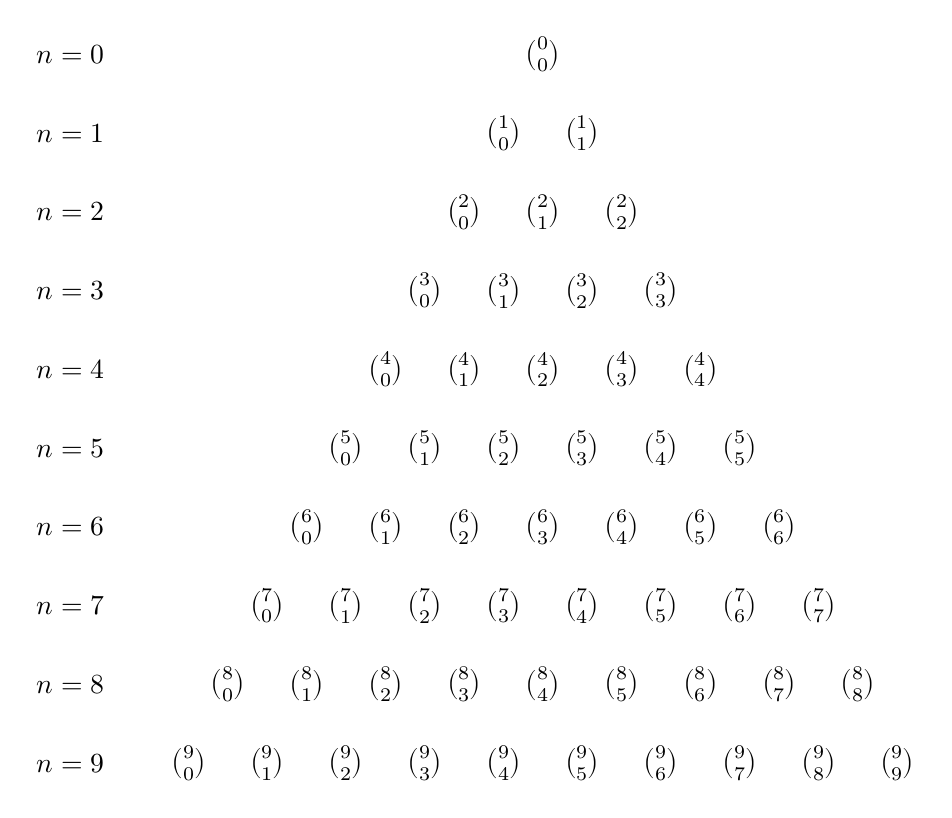
\begin{tikzpicture}
    \def\rowcount{9}
    \foreach \n in {0,...,\rowcount} {
    \node at (-6, -\n) {$n=\n$};
        \foreach \k in {0,...,\n} {
            % Tính giá trị hệ số nhị thức sử dụng hàm \binom của gói amsmath
            \node at (\k-\n/2, -\n) {$\binom{\n}{\k}$};
        }
    }
\end{tikzpicture}

\end{document}
